%% GENERATED by tools/from_docs.py from stepss-docs. Do not edit by hand:
%% edit the page named below in stepss-docs and regenerate.
%% source: stepss-docs/src/content/docs/test-systems/nordic.mdx

\chapter{The IEEE Nordic test system}\label{doc:ts-nordic}

The Nordic test system is a well-established benchmark for voltage stability and long-term dynamics studies, originally defined in the \href{https://resourcecenter.ieee-pes.org/publications/technical-reports/PESTR19.html}{IEEE PES Technical Report on Test Systems for Voltage Stability Analysis and Security Assessment}. It represents a realistic multi-area transmission network and is used extensively in research and education.

\begin{center}\rule{0.5\linewidth}{0.5pt}\end{center}

\section{System Overview}\label{ts-nordic:system-overview}

{\def\LTcaptype{none} % do not increment counter
\begin{small}\begin{longtable}[]{@{}
  >{\raggedright\arraybackslash}p{(\linewidth - 4\tabcolsep) * \real{0.4607}}
  >{\raggedright\arraybackslash}p{(\linewidth - 4\tabcolsep) * \real{0.5393}}
@{}}
\toprule\noalign{}
\begin{minipage}[b]{\linewidth}\raggedright
Property
\end{minipage} & \begin{minipage}[b]{\linewidth}\raggedright
Value
\end{minipage} \\
\midrule\noalign{}
\endhead
\bottomrule\noalign{}
\endlastfoot
Nominal frequency & 50 Hz \\
Buses & 74 \\
Synchronous generators & 20 (g1--g20) \\
Transformers & 50 (\texttt{TRFO} records, step-up and distribution) \\
Transmission lines & 52 \\
Voltage levels & 15 kV, 20 kV, 130 kV, 220 kV, 400 kV \\
Installed generation & 16,550 MVA (11,500 MW dispatched at operating point A) \\
\end{longtable}\end{small}
}

The system is divided into several areas interconnected through a meshed 400 kV transmission network. Lower voltage levels (130 kV, 220 kV) serve sub-transmission, while 15 kV and 20 kV buses connect generators and distribution loads.

\section{One-line Diagram}\label{ts-nordic:one-line-diagram}

\begin{figure}[htbp]
\centering
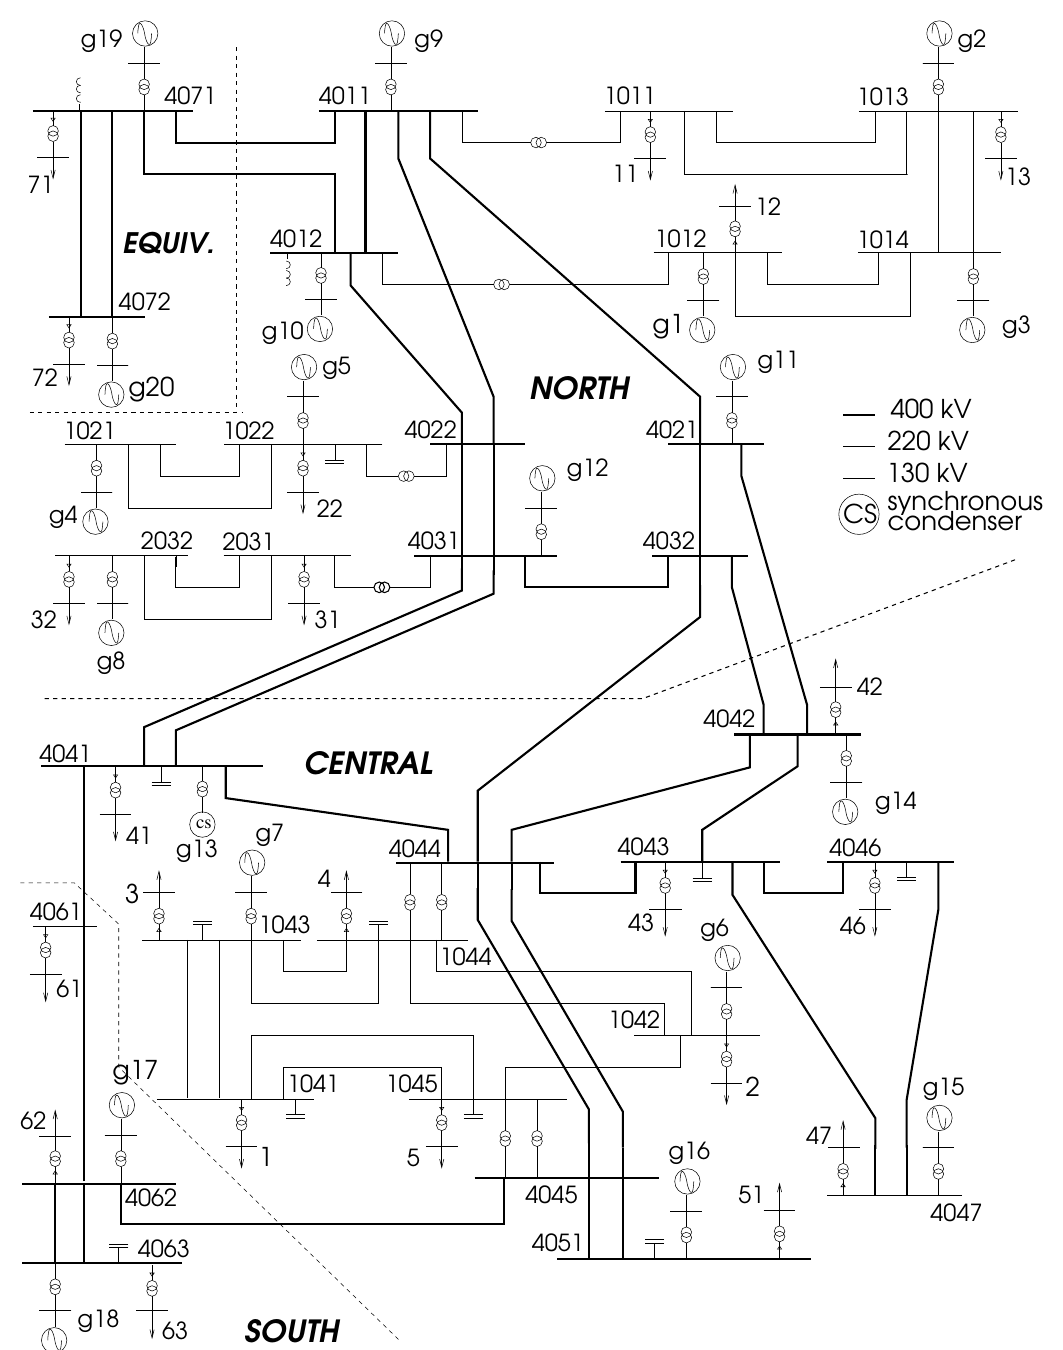
\includegraphics[width=0.75\linewidth]{figures/nordic_oneline}
\caption{One-line diagram of the IEEE Nordic test system (from the Nordic test system report, T.}
\end{figure}

\begin{center}\rule{0.5\linewidth}{0.5pt}\end{center}

\section{Dynamic Models}\label{ts-nordic:dynamic-models}

Each generator is modeled as a detailed synchronous machine (\texttt{SYNC\_MACH}) with:

\begin{itemize}
\tightlist
\item
  \textbf{Machine model}: Subtransient model with d- and q-axis dynamics (round-rotor or salient-pole depending on unit type)
\item
  \textbf{Excitation system}: \texttt{EXC\ GENERIC1}. a generic AVR with field current limiter, OEL, and optional PSS (SPEEDIN type)
\item
  \textbf{Governor/turbine}:

  \begin{itemize}
  \tightlist
  \item
    Hydro units (g1--g5, g8--g12, g19--g20): \texttt{TOR\ HYDRO\_GENERIC1}, hydraulic turbine with governor
  \item
    Thermal units (g6--g7, g13--g18): \texttt{TOR\ CONSTANT}: constant mechanical torque
  \end{itemize}
\end{itemize}

Loads are represented using the \texttt{INJEC\ vfd\_load} model (variable-frequency-dependent exponential recovery load) with voltage-dependent active and reactive power characteristics.

Under-load tap changers are modeled with \texttt{DCTL\ LTC2} discrete controllers on all distribution transformers.

\begin{center}\rule{0.5\linewidth}{0.5pt}\end{center}

\section{Operating Points}\label{ts-nordic:operating-points}

The repository provides two main operating points plus a family of load-increase variants:

{\def\LTcaptype{none} % do not increment counter
\begin{small}\begin{longtable}[]{@{}
  >{\raggedright\arraybackslash}p{(\linewidth - 4\tabcolsep) * \real{0.4439}}
  >{\raggedright\arraybackslash}p{(\linewidth - 4\tabcolsep) * \real{0.5561}}
@{}}
\toprule\noalign{}
\begin{minipage}[b]{\linewidth}\raggedright
File
\end{minipage} & \begin{minipage}[b]{\linewidth}\raggedright
Description
\end{minipage} \\
\midrule\noalign{}
\endhead
\bottomrule\noalign{}
\endlastfoot
\texttt{lf\_A.dat} / \texttt{dyn\_A.dat} / \texttt{volt\_rat\_A.dat} & Operating Point A, base case, moderately stressed \\
\texttt{lf\_B.dat} / \texttt{dyn\_B.dat} / \texttt{volt\_rat\_B.dat} & Operating Point B, heavily stressed, closer to voltage collapse \\
\texttt{lf\_B\_plus\_*.dat} / \texttt{volt\_rat\_B\_plus*.dat} & Operating Point B with total load increased by 25 to 500 MW \\
\end{longtable}\end{small}
}

Operating Point B is the primary case for voltage stability studies; it features higher load levels in the central area and reduced reactive power reserves. The \texttt{B\_plus} variants (documented in \texttt{doc/variants.pdf}) progressively stress the system further and are useful for tracing the loadability limit.

\begin{center}\rule{0.5\linewidth}{0.5pt}\end{center}

\section{Repository Contents}\label{ts-nordic:repository-contents}

{\def\LTcaptype{none} % do not increment counter
\begin{small}\begin{longtable}[]{@{}
  >{\raggedright\arraybackslash}p{(\linewidth - 4\tabcolsep) * \real{0.3362}}
  >{\raggedright\arraybackslash}p{(\linewidth - 4\tabcolsep) * \real{0.6638}}
@{}}
\toprule\noalign{}
\begin{minipage}[b]{\linewidth}\raggedright
Path
\end{minipage} & \begin{minipage}[b]{\linewidth}\raggedright
Description
\end{minipage} \\
\midrule\noalign{}
\endhead
\bottomrule\noalign{}
\endlastfoot
\texttt{lf\_*.dat} / \texttt{dyn\_*.dat} / \texttt{volt\_rat\_*.dat} & Load-flow data, dynamic data, and power-flow solutions for all operating points \\
\texttt{settings1.dat} & Solver configuration (time step, tolerances, threading) \\
\texttt{obs.dat} & Observation file, monitors all buses, branches, machines, injectors \\
\texttt{uvls.dat} & Undervoltage load-shedding (UVLS) controllers \\
\texttt{nothing.dst} & Empty disturbance file (undisturbed simulation) \\
\texttt{trip\_gen.dst} / \texttt{trip\_branch.dst} & Generator and branch trip disturbance scenarios \\
\texttt{short\_trip\_branch.dst} & Short-circuit followed by branch trip (\texttt{\_changeLTCs} variant modifies tap-changer behavior) \\
\texttt{eigen.dst} / \texttt{dampJac.dst} & Jacobian export runs for \hyperref[doc:eigenanalysis]{eigenanalysis} \\
\texttt{cmd.txt} / \texttt{sim\_*.cfg} & RAMSES command file and STEPSS GUI simulation configurations (\texttt{sim\_nothing}, \texttt{sim\_trip}, \texttt{sim\_short\_trip}) \\
\texttt{doc/} & Detailed system report (\texttt{Nordic\_test\_system\_V6.pdf}) and operating-point variants description (\texttt{variants.pdf}) \\
\texttt{jupyterhub-tutorial/} & Self-contained tutorial with \texttt{Execute.ipynb}, a step-by-step voltage collapse notebook \\
\end{longtable}\end{small}
}

\begin{center}\rule{0.5\linewidth}{0.5pt}\end{center}

\section{Disturbance Scenarios}\label{ts-nordic:disturbance-scenarios}

\subsection{\texorpdfstring{Generator Trip (\texttt{trip\_gen.dst})}{Generator Trip (trip\_gen.dst)}}\label{ts-nordic:generator-trip-trip_gen.dst}

Trips generator g2 at \(t = 1\) s and observes the long-term system response:

\begin{Verbatim}
0.000 CONTINUE SOLVER BD 0.020 0.001 0.0 ABL
1.000 BREAKER SYNC_MACH g2 0
100.000 STOP
\end{Verbatim}

\subsection{\texorpdfstring{Short-Circuit with Branch Trip (\texttt{short\_trip\_branch.dst})}{Short-Circuit with Branch Trip (short\_trip\_branch.dst)}}\label{ts-nordic:short-circuit-with-branch-trip-short_trip_branch.dst}

Applies a three-phase fault on bus 4032 at \(t = 1\) s, cleared after 100 ms by tripping the faulted branch:

\begin{Verbatim}
0.000 CONTINUE SOLVER BD 0.020 0.001 0.00 ABL
1.000 FAULT BUS 4032 0. 0.
1.100 CLEAR BUS 4032
1.100 BREAKER BRANCH 4032-4044 0 0
200.000 STOP
\end{Verbatim}

The \texttt{jupyterhub-tutorial/} folder contains its own variants of these scenarios (e.g.~with shunt compensation switching) used by the tutorial notebook.

\begin{center}\rule{0.5\linewidth}{0.5pt}\end{center}

\section{Quick Start}\label{ts-nordic:quick-start}

\subsection{Prerequisites}\label{ts-nordic:prerequisites}

\begin{itemize}
\tightlist
\item
  Python 3 with \hyperref[doc:py-install]{stepss} installed
\item
  JupyterLab (recommended) or any Python environment
\end{itemize}

Install stepss following the \hyperref[doc:py-install]{installation guide}.

\subsection{Running a Simulation}\label{ts-nordic:running-a-simulation}

\begin{enumerate}
\def\labelenumi{\arabic{enumi}.}
\item
  Clone the repository:

\begin{Verbatim}
git clone https://github.com/SPS-L/stepss-IEEE-Nordic-Test-system.git
cd stepss-IEEE-Nordic-Test-system
\end{Verbatim}
\item
  Open \texttt{jupyterhub-tutorial/Execute.ipynb} in Jupyter and run cells sequentially, or use the following Python script from the repository root:
\end{enumerate}

\textbf{Python Script}

\begin{Verbatim}
import stepss

case = stepss.cfg()
case.addData("dyn_B.dat")
case.addData("volt_rat_B.dat")
case.addData("settings1.dat")
case.addObs("obs.dat")
case.addDst("trip_gen.dst")

ram = stepss.sim()
ram.execSim(case, 150.0)

# Extract and plot results
ext = stepss.extractor(case.getTrj())
\end{Verbatim}

\textbf{Jupyter Notebook}

Open \texttt{Execute.ipynb} directly. It contains a complete guided tutorial with inline plots for:
- Bus voltage evolution
- Generator frequency deviations
- Governor valve output and mechanical power
- Active and reactive power output

\begin{center}\rule{0.5\linewidth}{0.5pt}\end{center}

\section{What to Observe}\label{ts-nordic:what-to-observe}

After a generator trip on Operating Point B, the simulation demonstrates:

\begin{itemize}
\tightlist
\item
  \textbf{Frequency transient}: immediate frequency drop followed by primary governor response from hydro units
\item
  \textbf{Voltage dynamics}: progressive voltage decline in the central area as load restoration (tap changers, thermostatic loads) increases demand beyond available reactive reserves
\item
  \textbf{Long-term voltage instability}: if the system lacks sufficient reactive support, voltages collapse over tens of seconds. a classic long-term voltage stability phenomenon
\end{itemize}

\begin{center}\rule{0.5\linewidth}{0.5pt}\end{center}

\section{License}\label{ts-nordic:license}

The \href{https://github.com/SPS-L/stepss-IEEE-Nordic-Test-system}{stepss-IEEE-Nordic-Test-system} repository is licensed under the \href{https://github.com/SPS-L/stepss-IEEE-Nordic-Test-system/blob/main/LICENSE}{Apache License 2.0}. The IEEE PES-TR19 report itself is not redistributed; obtain it from the IEEE Resource Center link below.

\section{References}\label{ts-nordic:references}

\begin{itemize}
\tightlist
\item
  IEEE PES Task Force on Test Systems for Voltage Stability Analysis and Security Assessment (chaired by T. Van Cutsem), ``Test Systems for Voltage Stability Analysis and Security Assessment,'' IEEE PES Technical Report PES-TR19, Aug.~2015. Available from the \href{https://resourcecenter.ieee-pes.org/publications/technical-reports/PESTR19.html}{IEEE Resource Center}
\item
  \href{https://sps-lab.org/project/stepss/}{STEPSS project page} at the Sustainable Power Systems Lab
\end{itemize}

\section{See Also}\label{ts-nordic:see-also}

\begin{itemize}
\tightlist
\item
  \hyperref[doc:py-examples]{Python API Examples}, Complete Python simulation workflow with this test system
\item
  \hyperref[doc:py-api]{Python API Reference}, Full API documentation for scripting simulations
\end{itemize}
